% !TeX root = ../../tesi.tex

Site 2 corresponds to the acquisition and inspection station dedicated to baked bread loaves. In contrast to Site 1, where RGB-D data are exploited to estimate volumetric properties of raw dough balls, Site 2 focuses on the visual analysis of the final baked product. The primary objective at this stage is the creation of a dedicated image dataset of baked loaves, followed by the training and deployment of the DEIMv2 object detection network for automated detection and anomaly-based quality assessment.

\subsection{Industrial Context and Monitoring Objectives}

At Site 2, the product has completed the baking process and is transported along the production line as finished bread loaves. At this stage, geometric variability is less critical than the overall visual appearance of the final product, including crust condition, browning patterns, and other surface irregularities. These characteristics may reflect deviations in baking quality and in the underlying process parameters.\\
The system deployed at Site 2 aims to:

\begin{itemize}
    \item Acquire a representative dataset of baked bread images,
    \item Train a dedicated DEIMv2 object detection model,
    \item Detect bread loaves in real time,
    \item Support anomaly-based quality monitoring of the final product.
\end{itemize}

\begin{figure}[h]
    \centering
    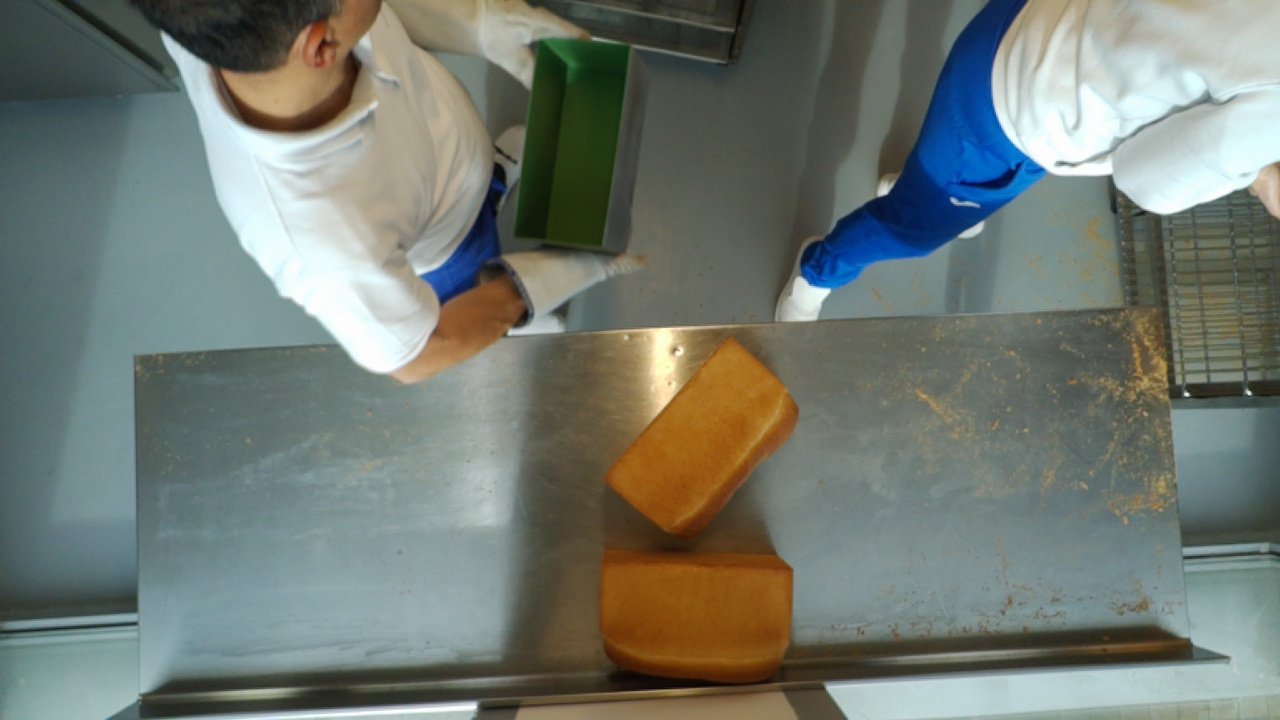
\includegraphics[width=0.65\linewidth]{images/Site2_breadloaf.jpg}
    \caption{Point of view of the Raspberry Pi Camera Module 3 Wide during the manual extraction phase, showing operators removing baked bread loaves from the trays under real production conditions}
    \label{fig:breadloaf}
\end{figure}

\subsection{Dataset Creation}

During the initial phase, the system operates in data acquisition mode. Following the same motion-triggered acquisition principle adopted at Site~1, images of baked bread loaves are captured by using background subtraction as an event trigger. At this site, the assessment is not based on depth cues but on visual characteristics such as color, illumination, and surface texture. For this reason, images are acquired under controlled lighting conditions to reduce visual variability due to the environment (see \emph{Practical challenges and system robustness} in Chapter~1) and to improve the consistency of both the collected dataset and the resulting analysis.

The collected dataset is subsequently annotated through an automatic labelling strategy based on Lang-SAM \cite{medeiros_luca-medeiroslang-segment-anything_2026} and used to train the DEIMv2 \cite{huang_real-time_2026} object detection network in an offline environment with higher computational resources. The details of the automatic labelling strategy and training procedure are described in Chapter~4.

This dataset creation phase is fundamental to ensure robustness of the detection model against variations in loaf shape, surface texture, illumination changes, and partial occlusions.

\subsection{Hardware Configuration}

Unlike Site 1, which relies on an RGB-D sensor and embedded GPU platform, Site 2 adopts a lightweight and cost-effective vision setup composed of:

\begin{itemize}
    \item A Raspberry Pi 5 \cite{raspberrypi_raspberry_pi_5_2026} for edge computation,
    \item A Raspberry Pi Camera Module 3 Wide \cite{raspberrypi_camera_documentation_2026} for RGB image acquisition.
\end{itemize}

The Raspberry Pi Camera Module 3 Wide provides a large field of view, enabling coverage of the table where the loaves are baked (as shown in Figure~\ref{fig:breadloaf}). Since volumetric estimation is not required at this stage, depth sensing is unnecessary, and a monocular RGB configuration is sufficient.

\subsection{Online Detection and Downstream Analysis}

Once training is completed, the DEIMv2 model is deployed on the Raspberry Pi 5 \cite{raspberrypi_raspberry_pi_5_2026} for inference. For each acquired RGB frame, the bread loaves are detected and the corresponding image regions are extracted. These regions are then passed to a downstream anomaly-detection stage for product-quality assessment. The detailed pipeline and anomaly-detection procedure are presented in Chapter~4.

\subsection{Role of Site 2 in the Overall Architecture}

Site 2 complements the functionality of Site 1 by extending the inspection framework from geometric analysis of raw dough to anomaly-based visual assessment of the final baked product. While Site 1 leverages RGB-D sensing for volumetric estimation, Site 2 employs a monocular RGB setup for anomaly detection on baked bread loaves.

Together, the two sites demonstrate the flexibility of the proposed DEIM-based architecture, which can be adapted to different sensing modalities and quality metrics while maintaining a consistent edge-computing paradigm.
